% TODO
% smoothed data
% Tmp calibration
% appendix sorting
% Peltier reference
% comments


\documentclass[10pt]{article}
\usepackage[utf8]{inputenc}
\usepackage{natbib}
\usepackage{graphicx}
\usepackage[margin=0.75in]{geometry}
\usepackage{url}
\usepackage{amsmath}
\usepackage{comment}
\usepackage[utf8]{inputenc}
\usepackage[T1]{fontenc}
%\usepackage[font={small,it}]{caption}
%\usepackage[font={it}]{caption}
%\usepackage{fancyhdr}
%\pagestyle{fancy}
%\fancyhf{}
%\lfoot{Iain Mclaughlan}
%\rfoot{s1524154}

\usepackage{listings}
\usepackage{color}
 
\definecolor{codegreen}{rgb}{0,0.6,0}
\definecolor{codegray}{rgb}{0.5,0.5,0.5}
\definecolor{codepurple}{rgb}{0.58,0,0.82}
\definecolor{backcolour}{rgb}{0.95,0.95,0.92}

\title{Precision Refrigerator}
\author{Iain McLaughlan\\ s1524154 }
\date{\today}

\begin{document}

\maketitle
\begin{abstract}
A precision refrigerator was built and controlled using a Raspberry Pi to precisely control the temperature of water by toggling the on/off state of a Peltier \cite{peltier}\cite{pelt} cooling unit. Different methods for determining the on/off state of the Peltier heat pump were used to converge the temperature of the water on an aimed temperature with different effectiveness. A scoring system was used to compare different convergence methods, and the advantages and disadvantages of each were compared. The devised methods are referred to by descriptor names. It was found that for an aim temperature of $21.4^oC$: `Converge' held a mean temperature of $21.4(1)^oC$ with $53.2(2)\%$ of the data falling within one reading error of the aim value ($\pm 0.0625^oC$). The more complex methods `Hysterisis Converge', `Rate Limit Convergence' and `Pre-emptive Convergence' each had means of $21.4(1)^oC$ and percentage scores of $62.6(2)\%$, $68.0(2)\%$ and $73.0(2)\%$ respectivly. The efficiency of this cooling unit was then tested, by comparing the energy consumed to change the temperature of the water with the specific heat capacity of water. The fridge was found to have a percentage efficiency of $6(1)\%$ when measured over $0.5$ and $1.0^oC$ temperature drops.
\end{abstract}

\section*{Introduction}
Microcontrollers can be used for a wide range of different applications. These applications, include embedded systems and can range from driving robots \cite{robomicro} to burglar detection \cite{microburg}. A microcontroller refers to a small computer that is usually based on a single integrated circuit. This single circuit often contains a central processing unit (CPU), some form of memory and usually some form of input/output (I/O) peripherals. In recent times microcontrollers, and in turn microprocessors, have become significantly more powerful and can control much more complex systems as a result.\\

One application of a microcontroller is in the fine control of a precision refrigerator. Here a microcontroller can use various inputs to control the temperature of various objects. Knowing, and being able to control, the temperature of objects with a high level of precision is very important in some fields. For example, during experiments looking at reactions at phase boundaries \cite{microfluidic} being able to precisely control the temperature to keep the substance at the desired level is very important in obtaining reliable results.\\

To precisely control the temperature of a substance it is useful to understand how much energy is required to heat and cool it. The energy required to change the temperature of a substance is determined by the heat capacity. The heat capacity ($C$) of a substance is defined as the ratio of heat transferred ($Q$) to or from the system and the resulting change in temperature ($T$) of the substance.  % The heat capacity is measured in $kJ/kg K$.

\begin{equation}\label{eq:heat_cap}
    C(T) = \frac{\delta Q}{dt}
\end{equation}

The heat capacity changes depending on the substance being heated. On top of this, the heat capacity also varies with temperature, and what variables are free to change and which are constrained i.e. constant pressure temperature changes vs constant volume temperature changes.\\

\begin{figure}[h!]
    \centering
    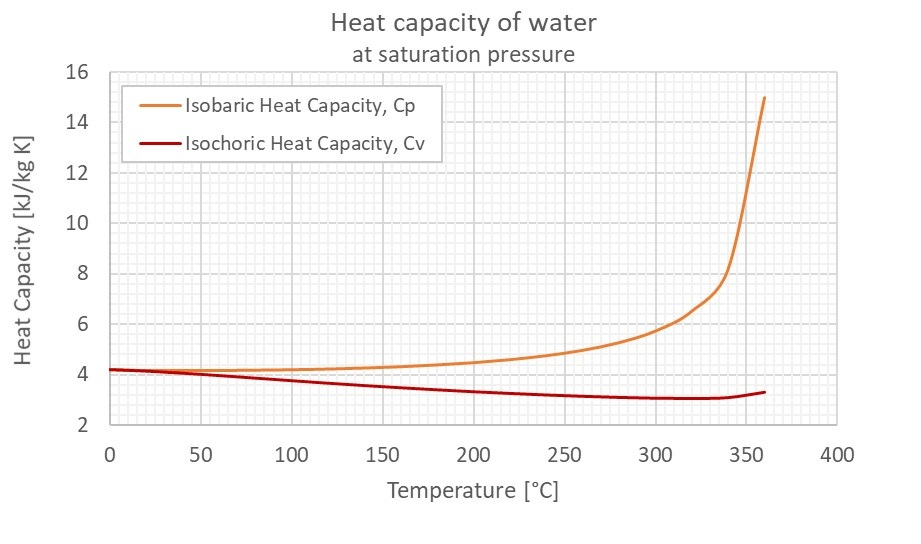
\includegraphics[scale=.75]{Heat_capacity_C.jpg}
    \caption{\it{The heat capacity of water varying differently when kept at constant pressure compared to being kept at constant volume \cite{heat_cap}.}}
    \label{fig:heat_cap_water}
\end{figure}

This variation can be seen in Figure \ref{fig:heat_cap_water}, where the heat capacity of water varies differently depending on which state variable is kept constant (either pressure or volume). \footnote{At temperatures close to $0^oC$ the values of heat capacity, Cp and Cv are approximately equal and only noticeably start to diverge from one another at temperatures close to $50^oC$.}\\

The energy required to change the temperature of the substance, along with the amount of energy used in total, can be used to calculate the efficiency of the cooling system. Efficiency is defined as the ratio of the useful work produced to the total energy expended. In the case of a refrigerator, this is the ratio of the energy supplied to the cooling unit compared to the energy actually used to cool.\\

\begin{figure}[h!]
    \centering
    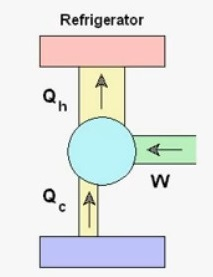
\includegraphics[scale=.75]{ref.jpg}
    \caption{\it{Energy movement through a refrigerator system, transferring heat (Qc) from a cold source ($T_{cold}$) by providing work energy (W) to drive the heat (Qh) to the hot sink ($T_{hot})$ \cite{fridge}.}}
    \label{fig:fridge}
\end{figure}

Refrigerators operate by supplying work to move heat from a cold source to a hot sink. The flow of heat for this process can be seen in Figure \ref{fig:fridge}. The efficiency ($\eta$) of the refrigeration process is given by;
\begin{equation}\label{eq:eff}
    \eta = \frac{Q_C}{Q_H-Q_C}=\frac{Q_C}{Q_H/Q_C - 1}
\end{equation}
The ideal circumstance, where all of the work available is used to move heat, is given by the Carnot efficiency \cite{carnot}. In this idealised case, the efficiency is purely determined by the temperature ($T$) of the heat reservoirs.
\begin{equation}\label{eq:carn_eff}
        \eta_c = \frac{T_C}{T_H-T_C}=\frac{T_C}{T_H/T_C - 1}
\end{equation}
This is an idealised case describing the maximum efficiency. In reality it is impossible, due to heat loss and friction, to reach this efficiency. 


% RPI Not a micro processor or micro controller but system on chip


\section*{Aims}
\begin{itemize}
    \item Build a circuit controlled by python code running on a Raspberry Pi that measures the temperature of a mass of water and can control the on/off state of a Peltier heat pump \cite{peltier}\cite{pelt} to control the cooling of the water. 
    \item Construct several convergence methods which determine the required on/off state of the Peltier depending on given inputs and compare their abilities at precisely controlling the temperature of the water.
    \item Measure the efficiency of the cooling circuit when reducing the temperature of a fixed mass of water by a known amount.
\end{itemize}
\section*{Method}
The Peltier heat pump cooling chip was controlled using a breadboard circuit built using a Raspberry Pi \cite{rpi} as a system on a chip microcontroller. The chip was powered using an external power supply, which was connected and disconnected using a transistor. A python script was written to control the state of the transistor depending on temperature readings from a thermometer. A link to this code can be found in Appendix \ref{app:code}

\subsection*{Thermometer Calibration}
The circuit was initially set up with a Programmable Resolution 1-Wire Digital Thermometer (DS18B20) \cite{thermometer}. This thermometer has a programmable precision of 9 to 12 bits and an accuracy of $\pm 0.5^oC$. In 12 bit mode, this gives the thermometer a highest precision where it is able to read at $2^{-4o} C (0.0625^o C)$. This was tested with a short python script which reads the temperature of the thermometer at regular time intervals. A second thermometer was connected in parallel with the first and was tested in the same way. Over a period of 200 seconds with the thermometer probes measuring the temperature of the water. The temperature from both thermometers was recorded.

\subsection*{Peltier Setup}
The Peltier was connected to a GwInstek GPS-x3303 power supply \cite{powe_sup}. This was in turn connected to a Darlington T0220 Transistor \cite{trans} which acted as a switch and could be controlled by a Raspberry Pi by toggling the state of one of its GPIO (general purpose input output) pins between a high and a low voltage. When the input voltage to the transistor was high the transistor switched on, which completed the Peltier circuit activating the cooling chip using the power supply. When the voltage was low the transistor switched off which disconnected the Peltier circuit and stopped the cooling chip from receiving power.\\

\begin{figure}[h!]
    \centering
    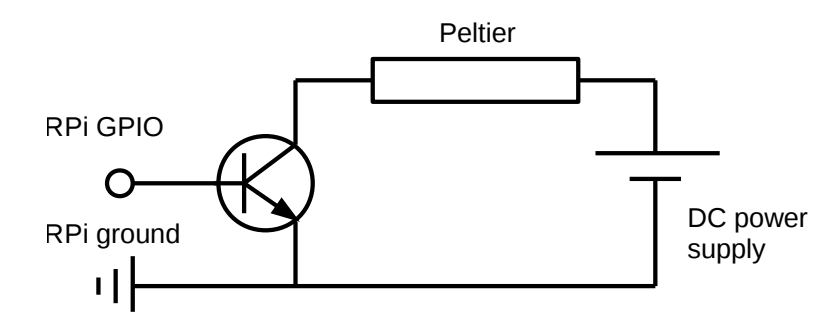
\includegraphics[scale=0.5]{circuit.png}
    \caption{\it{Circuit diagram showing the Peltier chip being powered by a DC power supply and controlled by a transistor switch whos state is determined by a RPi \cite{course_notes}.}}
    \label{fig:circuit}
\end{figure}

The cooling chip circuit was tested by toggling on and off the transistor with the power supply set to a low voltage and current. The chip was held to check that one side heated as the other side cooled when powered. This was only done in short bursts as leaving the chip running for long periods of time when not connected to a heat sink can damage the chip. \\

Once the Peltier and thermometer were working and tested the Peltier chip was placed on a heat sink. On top of this a small beaker was placed, filled with $50ml$ of water and a thermometer probe was used to measure the temperature of the water. A second thermometer was set up to read the ambient room temperature near the water beaker. To help gain an understanding of how the water heats and cools a prolonged cooling phase ($\sim15$ minutes) was recorded and plotted to see the trend. Following this, the water was then left to heat for the same time and was again plotted to see the trend.


 % **** Set up diagram? ****

\subsection*{Controlling the Cooling Chip}
Several methods were used to determine the required state of the cooling chip, which aimed to converge the temperature of the water down to a target temperature. In all methods, a precision range was set which corresponded to the precision with which the thermometer could measure (in some cases this was increased to see different responses). This was done to allow for inaccuracies in the temperature readings, prevent the cooling chip from rapidly switching on and off, which could damage it, and provide an acceptable range, around the aim temperature, which would be counted as the same as the aim temperature (aim temperature $\pm$ precision = aim temperature).\\

These methods worked using the following rules:\\ % converge(), hysteretic_conv(), rate_limit_conv(), pre_empt_conv()

1 Converge (Converge). If the temperature of the water was above the aim temperature plus the precision then the chip was switched on. Alternatively, if the temperature of the water was below the aim temperature minus the precision then the chip was turned off.\\

2 Hysteresis Convergence (Hysteretic$\_$conv). It was observed that the rate of heating from the ambient temperature was greater than the rate of cooling from the chip. This resulted in the the cooling phase lasting longer than the heating phase. To combat this, the cooling chip was activated when the temperature was above the aim temperature plus a proportion of the precision level. This reduced the relative heating phase limiting the temperature overshoot.\\

3 Rate Limit Convergence (Rate$\_$limit$\_$conv). Given the observation above, that the rate of heating from the ambient temperature was greater than the rate of cooling from the chip, the high-end temperature limit where the chip is turned on was adaptively moved depending on the difference between the ambient temperature and the aim temperature. If the room temperature is much higher than the aim temperature then the assumption is that the rate of heating will be very fast, so the chip is turned on at a lower temperature than it would if the temperature difference was less. This should limit the overshoot of the temperature in the heating phase by changing the upper limit depending on the expected rate of temperature increase from the surroundings. \\

4 Pre-emptive Convergence (Pre$\_$empt$\_$conv). Here the rate of temperature change was used to try and pre-empt the point at which the temperature will become greater than, or less than, the aim temperature, and toggle the state of the cooling chip accordingly. This is done using the idea that the temperature of the water will continue to change even after the state of the chip has been changed. For example, when the water is heating, if the rate ($^oC/s$) added to the current temperature will be greater than the aim temperature then the cooling chip will be turned on to start the cooling process before the temperature has fully risen to the aim temperature. This rate can be multiplied by an estimated change factor i.e number of seconds for an effect to be realised, to try and work closer to the aim temperature.\\

To compare the different convergence methods a scoring system was devised which looks at temperature measurements over a test period and finds the fraction of these which were within the precision range of the desired temperature. The test range was chosen to only start when the temperature had first reached the aim temperature so as to only count readings in the region around an aim temperature and not while initially cooling from the original temperature to the aim temperature.   \\

In addition to this, the efficiency of the cooling system was measured. This measurement was made during the initial cooling phase before the aim temperature had been reached for the first time. This was done by recording the time ($t$) between when the chip was first turned on and when the aim temperature was reached. This time was multiplied by the power provided from the power source ($P=IV$) to give a total energy used to cool. This was then compared to the energy required to cool the water by the same temperature difference ($\Delta T$) using the known specific heat capacity ($c$) and mass ($m$) of the water. The ratios of these energies were used to find the efficiency of the overall cooling system:
\begin{equation}
    \eta_{sys} = \frac{\text{Energy To Cool Water}}{\text{Total Energy Supplied}} = \frac{cm\Delta T}{Pt}
\end{equation}


% using the heat capacity of water at room temp
\section*{Results and Discussion}
An important thing to note throughout this results section is that the precision of the thermometer in its most precise setting is $0.0625^oC$. This precision is the reason behind the step-like nature in the raw data. Attempts were made to smooth the data, which can be seen in Appendix \ref{app:smoothed}, however this was felt to potentially distort changes in aiming to display smoother data. Instead of smoothing data the decision was made to run experiments over long periods of time, which will show trends over the step-like nature of the temperature readings. \\

\subsection*{Thermometer Calibration}
The readings from two thermometers submerged in water close to one another were measured simultaneously. These temperature data were plotted and shown in Figure \ref{fig:therm_calib}.
\begin{figure}[h!]
    \centering
    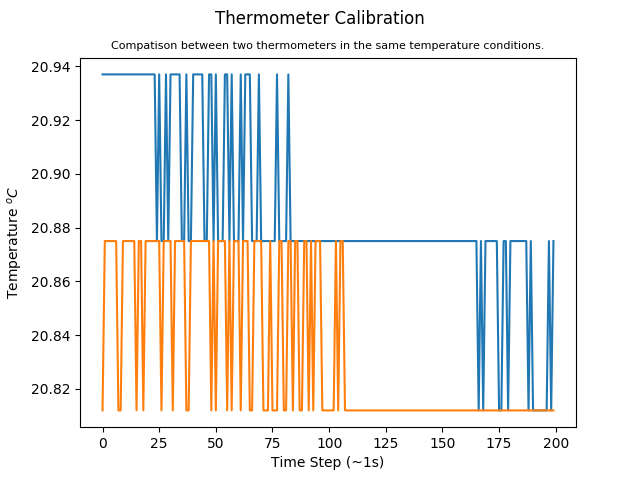
\includegraphics[scale=0.75]{therm_calib.png}
    \caption{\it{Thermometer calibration data measured from two separate thermometers in water.}}
    \label{fig:therm_calib}
\end{figure}

It can be seen looking at this that the temperature reading from the blue thermometer is consistently somewhere between one level of precision and equal to the temperature being read from the orange thermometer. The mean temperature from each data set was found and was $20.886^oC$ and $20.834^oC$. These values agree with each other within the level of precision of the thermometers ($0.0625^oC$) and comfortably within the $0.5^oC$ accuracy of the thermometers used \cite{thermometer}. To confirm these levels of agreement over the working temperature range used, the temperature was cooled to slightly below the working range and the same measurements were taken. These can be seen in Appendix \ref{app:therm_calib}. These results were found to be consistent with the ones shown here, showing that there were no noticeable discrepancies between the two separate thermometer readings over the range of temperatures used for experimental measurements.
Since these values agree with each other within one $\sigma$ it was assumed that the temperatures were the same and no alteration was needed for future temperature measurements. A slight alteration could have been made to bring the temperatures to a more consistent average value i.e $blue - 0.5\times(T_{blue}-T_{orange})$ and the opposite for the orange data, however, since the following experiments are focused on the concept of convergence about a point, rather than the exact temperature achieved, this was not done.

\subsection*{Cooling and Heating Data}
The cooling and heating data was recorded over 2000 data points which can be seen in Figure: \ref{fig:heat_and_cool_curve}. These show an exponential decay when cooling and an exponential increase when heating. Throughout the recording process, the ambient lab temperature steadily increased from $22.62^oC$ to $24.27^oC$, due to the presence of others working in the same room. Note, the water temperature is consistently slightly below room temperature even after being left for a long period of time.\\

\begin{figure}[h!]
    \centering
    \subfloat{{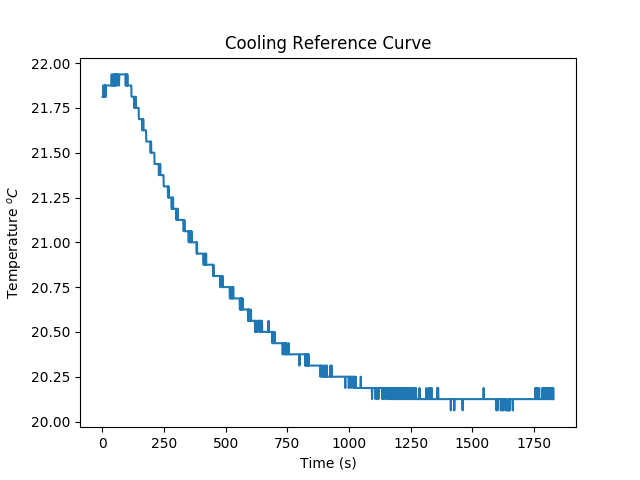
\includegraphics[width=8.45cm]{Cooling_data_curve_long.png} }}%
    \qquad
    \subfloat{{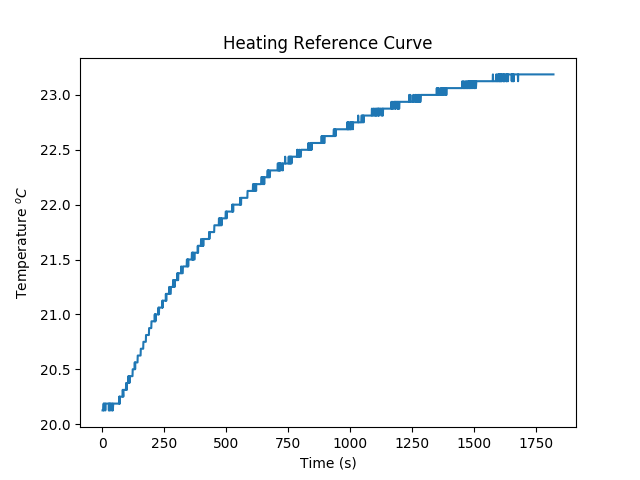
\includegraphics[width=8.45cm]{Heating_data_curve_long.png} }}%
    \caption{\it{Cooling and heating curves consisting of 2000 data points each. Each data point corresponds to $\sim 1$ second ($0.89$ seconds). }}%
    \label{fig:heat_and_cool_curve}%
\end{figure}

Cooling and Heating data recorded over 1000 data points rather than 2000 can be seen in Appendix \ref{app:short_data}. Comparing these shows that it takes a significant time for the temperature to reach its limiting point where the graph begins to plateau. Over short periods of time ($\sim 1$ minute) the rate of temperature change is constantly varying.\\

From the cooling data, it can be seen that the Peltier heat pump chip can only cool the water by around $1.8^oC$ below its initial temperature. This provides slight limitations later as operating at lower temperatures could give the possibility of working with a heating curve that is approximately linear over the working range. This could allow predictions to be made more readily of how quickly the water will heat. The same can not be done in reverse i.e. having a higher operating temperature to have an approximately linear cooling line due to the limitations of relying on the room temperature to act as a heater. When working close to the room temperature the relative heating is very slow and not easy to predict or measure given the precision of the thermometer readings. Having either a larger or more powerful cooling chip could allow work at lower temperatures and make these approximations possible. \\

A further possible use for this data would be to use the curves to predict how quickly the temperature will change when at a given temperature. This is not possible in this instance due to the room temperature not being constant throughout. Even if the data were corrected to represent degrees below room temperature, this would still not work as the efficiency of the cooling chip will change depending on the working temperatures. The Peltier cooling chip's efficiency will be limited due to the principles from equations \ref{eq:eff} and \ref{eq:carn_eff}. To control this the temperature difference between the bottom of the water beaker and the temperature of the top of the heat sink would have to be relatively constant. On top of this, the Peltier chip will have its own working efficiency which will limit this method of temperature change predictions.

\subsection*{Convergence Methods}
Throughout each of these method tests, measurements were made over 500 time steps (which correspond to about 1 second each). For each method, the average temperature was found. A reduced $\chi^2$ value was obtained by comparing to an optimum straight line fit at the optimum temperature. And a percentage score for what percentage of the data points fall within one reading error of the thermometer from the aim temperature (aim temperature $\pm 2^{-4}$). For each set of readings, the aim temperature was set to $21.4^oC$ and the starting room temperature for each was recorded.\\
\newpage
\subsection*{Converge}
Here the cooling chip was toggled on and of if the water temperature was above or below the aim temperature of $21.4^oC$. \\

\begin{figure}[h!]
    \centering
    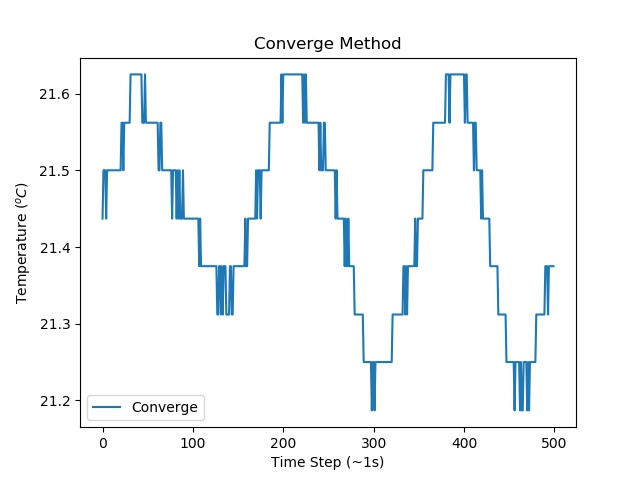
\includegraphics[scale=0.75]{converge.jpg}
    \caption{\it{The steady state oscillations of the `Converge' method about an aim temperature of $21.4^oC$.}}
    \label{fig:conv}
\end{figure}

It can be seen that the temperature of the water oscillates about the aim temperature in a sinusoidal manner where the temperature overshoots the aim temperature fairly evenly when both increasing and decreasing in temperature. \\

The average temperature over the 500 measurements was $21.4(1)^oC$. A total error was found by combining the thermometer precision with the standard deviation about the mean ($\sigma$), giving a value of the total error to be, $0.14^oC$. The reduced $\chi^2$ of the data when fitted to an ideal temperature, (a horizontal line at the aim temperature) was found to be, $0.29$ which is significantly less than 1, leading to the assumption that the data has been overfitted relative to the error. This method of convergence maintained the water temperature, within the precision level of the thermometer, of the aim temperature $53.2(2)\%$ of the time \footnote{Examples of the calculations used to find these values can be seen in Appendix \ref{app:errors}.}.\\

\subsection*{Hysteresis Convergence}
Here the point at which the cooling chip was turned on was brought down so that the heating time was reduced compared to the cooling time to try and combat the effect of the rate of heating being faster on average than the rate of cooling.\\ 

\begin{figure}[h!]
    \centering
    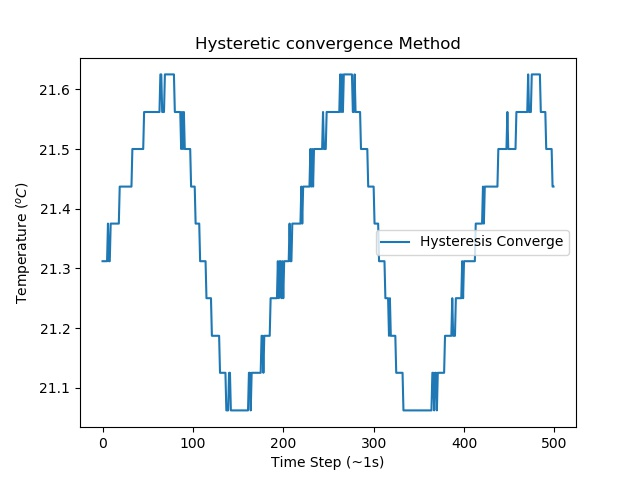
\includegraphics[scale=0.75]{hyst_conv.jpg}
    \caption{\it{The steady state oscillations of the `Hysteretic$\_$conv' method about an aim temperature of $21.4^oC$.}}
    \label{fig:hyst}
\end{figure}

This gave a mean value of $21.4(2)^oC$, which is equivalent to `Converge'. This method gave a reduced $\chi^2$, when fitted to the aim temperature, of $0.55$ which indicates a larger spread of data when again compared to `converge'. The changes in the cooling and heating phases result in a smaller frequency of oscillation when compared to other methods. This could have benefits if the cooler used became less efficient when switched on and off rapidly, but instead operates better when either on or off for more prolonged periods of time. This method gave a percentage score of $62.6\%$ which controls the temperature more precisely than the baseline convergence method used above.\\
% \newpage

\subsection*{Rate Limit Convergence}
Similarly to the hysteretic method above the upper limit at which the cooling chip is turned on is actively changed dependent on the difference between the aim temperature and the current room temperature. If there was a big temperature difference, with the room temperature being much greater, then it was assumed that the heating rate would be relatively quicker than if this difference was low. To combat this, the upper limit was set to be smaller with higher temperature differences and larger when the heating rate due to the ambient temperature was slow.\\

\begin{figure}[t]
    \centering
    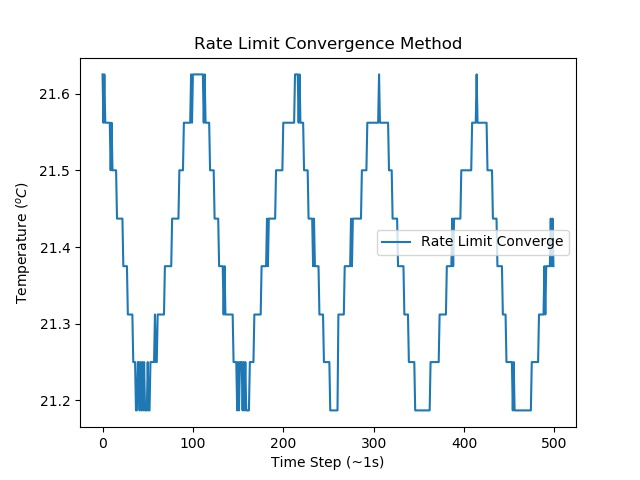
\includegraphics[scale=0.75]{rate_lim.jpg}
    \caption{\it{The steady state oscillations of the `Rate$\_$limit$\_$conv' method about an aim temperature of $21.4^oC$.}}
    \label{fig:rate}
\end{figure}

Here the average value was $21.4(1)^oC$ with a reduced $\chi^2$ about the aim of $0.29$. These results are very comparable to the previous two methods, however, more significant differences can be found when looking at the percentage score, which showed that the temperature was within the precision of the thermometer $68.0(2)\%$ of the time. It can also be seen that the frequency of oscillation here is larger. Here there are approximately 4.75 full oscillations in the 500 measurements compared to the approximately 2.75 for `Converge' the reasoning behind this is unclear. A possible explanation is that the chip is being controlled by a more advanced control system so the temperature is actually being controlled with more precision, however, this is not being fully shown due to the limitations of the precision of the thermometer.\\
\newpage
\subsection*{Pre-emptive Convergence}
The state of the chip was controlled here by looking at the rate of temperature change over the last few steps, and if that rate would carry the temperature over the aim temperature then the state of the Peltier was pre-emptively toggled to the opposite state.\\

\begin{figure}[h!]
    \centering
    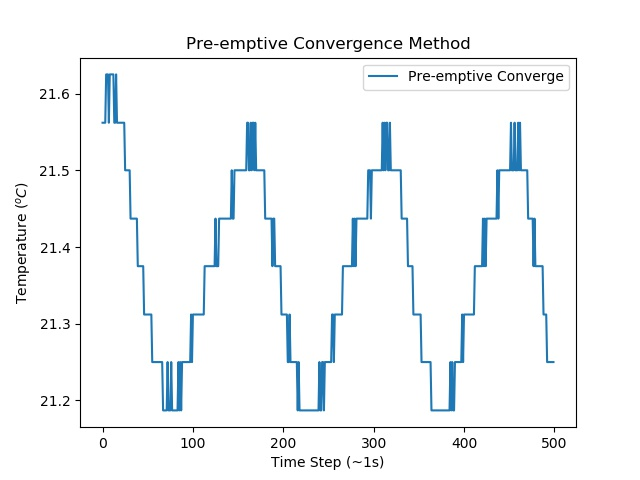
\includegraphics[scale=0.75]{pre_emp.jpg}
    \caption{\it{The steady state oscillations of the `Pre$\_$empt$\_$conv' method about an aim temperature of $21.4^oC$.}}
    \label{fig:pre}
\end{figure}

This method gave a mean value of $21.4(1)^oC$ and a reduced $\chi^2$ about the aim temperature of 0.24. The $\chi^2$ result is very similar to those seen previously along with a consistent average temperature across the 500 measurements. This method again steps up the percentage of data within the range about the aim to $73(2)\%$. This is the only method where the improved convergence about the aim can be reasonably seen by eye when comparing the graphs shown in Figures \ref{fig:conv}, \ref{fig:hyst}, \ref{fig:rate} and \ref{fig:pre}. Here the temperature on the high end sits on a precision level lower than the other methods showing that the method keeps the temperature closer to the aim. A graph showing all of the plots overlaid on top of one another can be seen in Appendix \ref{app:comparison}, where some of the differences between plots can be seen more easily.\\

Overall the convergence methods can be seen to be fairly comparable when viewed by eye and only by looking deeper into the effectiveness of each method, mainly through the use of the percentage score, can a meaningful difference be seen. In the case where a cooling chip is used where the efficiency of the chip may be compromised by toggling on and off more rapidly, it may be beneficial to use a convergence method similar to that of the `Hysteresis Convergence' due to the lower frequency of oscillation of the temperature. However, if this is not an issue the other methods like the rate limiting and pre-emptive methods control the temperature about an aim with a higher level of precision. The pre-emptive method used was rough in the sense that assumptions were made about how long it would take for a change in state to make a difference to the temperature of the water. These values could be tuned through more trial runs to further improve this method.

\subsection*{Cooler System Efficiency}
The efficiency of the cooling system was measured by finding the ratio of the energy required to cool $50ml$ of water by the given temperature change to the energy supplied to the system from the power supply. These results were taken when cooling over different ranges from room temperature. throughout these calculations the heat capacity of water was taken to be constant at a value of $4.182KJkg^{-1}K^{-1}$\cite{heat_cap_val} and the input voltage and current from the power supply were $3.0V$ and $1.5A$ respectively. \\

\begin{table}[h!]
    \centering
    \begin{tabular}{|c|c|}
        \hline
        Efficiency ($\%$) & Cooling Range from room temperature ($^oC$) \\
        \hline
        8.24 & 0.5 \\
        4.00 & 0.5\\
        11.81 & 0.5 \\
        3.08 & 1.0\\
        3.65 & 1.0\\
        8.81 & 1.0\\
        \hline 
    \end{tabular}
    \caption{\it{Cooling system percentage efficiencies when cooled to a certain change below room temperature.}}
    \label{tab:efficiencies}
\end{table}

Here in table \ref{tab:efficiencies} it can be seen that the mean efficiency of the system overall measurements was $6.60\%$ with a random error of $1.45\%$. The temperature drops, when compared to room temperature, were recorded as it was thought that because the cooling rate slows at lower temperatures which can be seen in Figure \ref{fig:heat_and_cool_curve} the efficiency of the cooling unit would decrease when cooled to lower temperatures. This is shown to be correct by the efficiency of the cooling unit being significantly less when cooling over $1^oC$ when compared to cooling by $0.5^oC$. When the water was cooled by $1^oC$ the mean efficiency was found to be $5(2)\%$. When cooled by $0.5^oC$ the mean efficiency was $8(3)\%$.\\

The efficiency of the overall system is very low, when compared to a domestic fridge which typically have efficiencies of around $40\%$ \cite{fridge_lit}. This is a result of many factors: The water that is cooled will gain heat from the surroundings at the same time. Not all of the cooling power of the Peltier will be transferred directly to the water. Some will go to the surroundings and some to the beaker. On top of this, temperature of the heat sink will increase with time as the cooling chip is on. This will reduce the temperature difference between the hot and cold reservoirs. In turn, this will reduce the maximum possible (Carnot, equation \ref{eq:carn_eff}) efficiency which will reduce the maximum realistic possible efficiency observed of the cooling system. If the temperature of the heat sink was kept constant by the addition of a powered fan or another method then the maximum possible efficiency would decrease less with time. However the addition of a fan would introduce a higher power consumption of the overall system. 

\newpage
\subsection*{Discussion}
On top of the reasons, limitations and area of improvement already discussed there are a few others which do not directly relate to the methods above.\\

The heat energy of the water will not be evenly distributed throughout the beaker. The water closest to the Peltier and closest to the sides of the beaker will be cooler than the water at the top of the beaker and far away from the Peltier. The heat will most probably be distributed throughout the sample by convection currents \cite{conv_cur}. This process takes time to distribute the energy throughout the sample so there will be a temperature gradient in the water. This could be improved by stirring the water. There are some issues with this as this will add an unknown amount of energy to the system.\\

The efficiency of the heat transferred from the cooling unit could be improved by adding a powered fan as discussed above to maintain the temperature of the heat sink. Thermal paste \cite{paste} could also be used. This would increase the efficiency of the heat being transferred as this would remove the air interface between the beaker and the Peltier and between the Peltier and the heat sink, replacing it with a much more thermally conductive material. The whole system could also be placed inside a calorimeter \cite{calorimeter} which is a highly insulated container where the energy from the surroundings can be reduced leaving the main cause of energy change is due to the energy added or removed.\\

\section*{Areas of Further Research}
Throughout the experimental process, a few areas could not be fully explored due to equipment and time limitations. Given more time it would be interesting to investigate the following: \\

Measuring the temperature using a higher precision thermometer. This would give smoother plots and make the differences between convergence methods more visually obvious.\\

Exploring methods for calculating the rate of heating and cooling from a standard heating and cooling curve for a given system. This could allow for more accurate predictions to pre-empt the temperature changes and therefore more intelligently control the state of the cooler. \\

Operating at lower temperatures with a higher power cooling device (or more efficient). Similarly to what has just been discussed with relying more on standard heating and cooling curves, operating at lower temperatures along with a higher power cooling device will increase the rates of heating and cooling allowing these to be approximated as linear and therefore easier to determine the change in temperature expected at the next time steps.\\

Another convergence method that was tried but not fully tested was one of pulse width modulation where the time that the cooling chip was on in a given period of time would reduce as the temperature came closer to the aim temperature. This was not fully tested as the Peltier's efficiency dropped significantly when being turned on and of rapidly. This method would however provide a way of asymptotically reducing the temperature and never going below the desired temperature which could be of use in certain applications.

% pulse width modulation and optimizing pre-empt  Appendix about smoothing
\section*{Conclusion}
A circuit was built that read the temperature of a sample of water and depending on what this temperature was in relation to an aim temperature then the on/off state of a Peltier heat pump was changed in order to raise or lower the temperature of the water to converge on the set aim temperature. This process was controlled using a Raspberry Pi as a system on a chip microcontroller. Four different convergence methods were tested in the following ways: by measuring the average temperature of the water over a long period of time and comparing this to the aim value; A reduced $\chi^2$ value for the data when compared to an ideal case where temperature $T=T_{aim}$; and a percentage score was found as the ratio of data which fell within one $\sigma$ of the aim temperature to those that did not. These methods were; Converge, Hysteresis Convergence, Rate Limit convergence and Pre-emptive Convergence. All of these methods held the average temperature at $21.4(1)^oC$ when set with an aim temperature of $21.4^oC$ over a prolonged period of time. The methods gave $\chi^2_{red}$ of 0.27, 0.55, 0.29 and 0.24 respectively. All of these are significantly less than one leading to the assumption that the data is overfitted to the ideal case. The most effective method of comparing these different methods was to find a percentage score which gave results of $53.2(2)\%, 62.6(2)\%, 68.0(2)\%$ and $73.0(2)\%$. This shows that more complex control systems such as Rate Limit Convergence and Pre-emptive Convergence are significantly better at precisely controlling the temperature than more basic methods. Lastly, the efficiency of the overall cooling system was measured by comparing the energy required to cool the water by a given amount to the total energy supplied from the power supply to create that cooling effect. This was found to be $8(3)\%$ when cooling to $0.5^OC$ below the waters steady room temperature and $5(2)\%$ when cooling by $1^oC$. 

\bibliographystyle{unsrt}
\bibliography{references}



\newpage
\appendix
\section{Cooling and Heating Reference Curves} \label{app:short_data}
\begin{figure}[h!]
    \centering
    \subfloat{{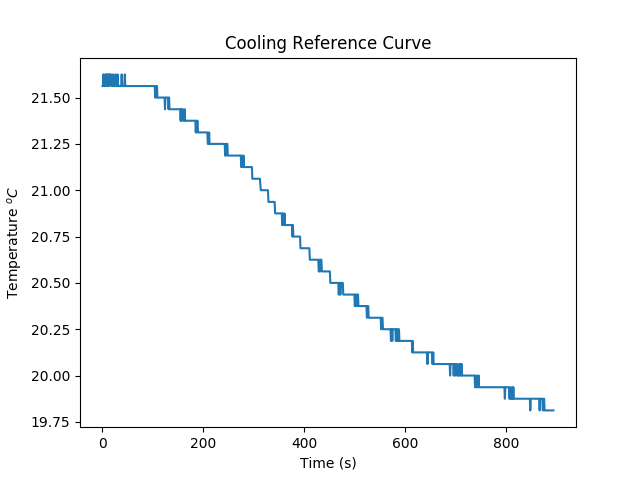
\includegraphics[width=8.45cm]{Cooling_data_curve_short.png} }}%
    \qquad
    \subfloat{{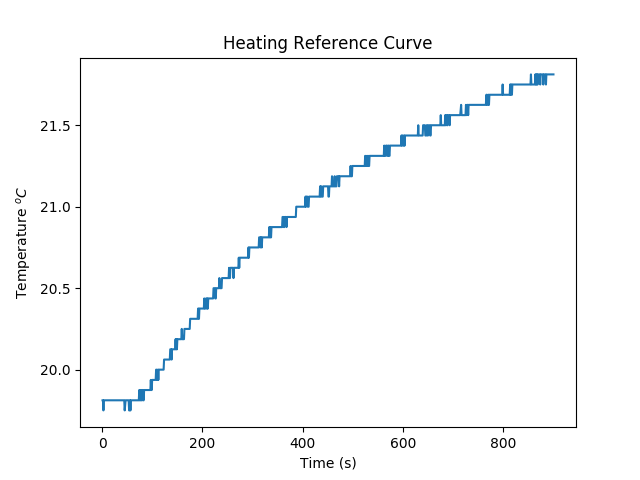
\includegraphics[width=8.45cm]{Heating_data_curve_short.png} }}%
    \caption{\it{Cooling and heating curves consisting of 1000 data points each. Each data point corresponds to $\sim 1$ second ($0.89$ seconds). }}%
    \label{fig:heat_and_cool_curve}%
\end{figure}

\section{Thermometer Calibration}\label{app:therm_calib}
\begin{figure}[h!]
    \centering
    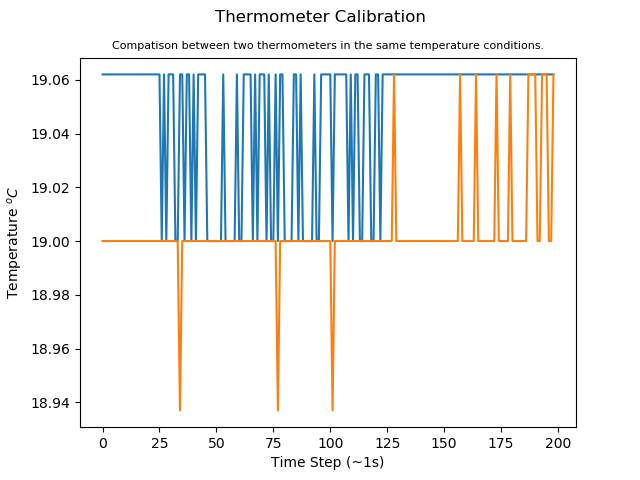
\includegraphics[scale=0.75]{therm_calib_low.png}
    \caption{\it{Thermometer calibration plot between two thermometers submerged in water at a temperature slightly below the working range for the measurements.}}
    \label{fig:therm_calib}
\end{figure}
\newpage
\section{Data Smoothing}\label{app:smoothed}

\begin{figure}[h!]
    \centering
    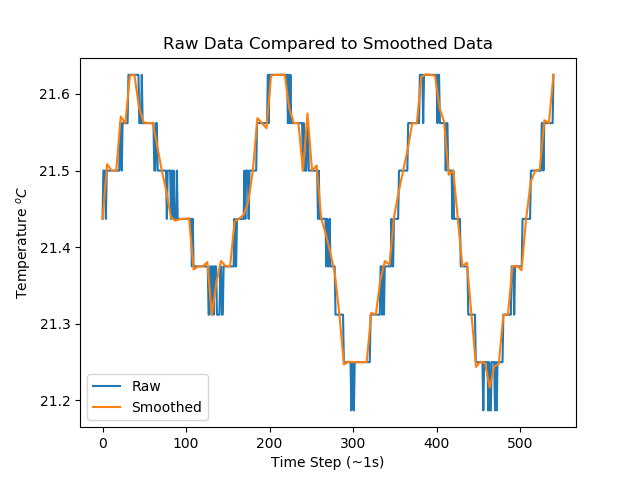
\includegraphics[scale=0.75]{raw_vs_smoothed.png}
    \caption{\it{Showing a comparison between raw and smoothed data. It can be seen that this method of smoothing the data does not add much value to the plot but in some cases overestimates the effects and in others underestimates.}}
    \label{fig:raw_vs_smooth}
\end{figure}

\section{Error Analysis}\label{app:errors}
\subsection{Total Error}
\begin{equation}
    \sigma^2 = \sum \frac{(x_i - \mu)^2}{N}
\end{equation}
\begin{equation}
    \sigma_{total} = \sqrt{\sigma^2 + \sigma_{therm}^2}
\end{equation}
Here $\sigma_{total}$ is the combined error; $\sigma^2$, the standard deviation; and $\sigma_{therm}$ the precision of the thermometer which had a value of $0.0625^oc$.
\subsection{Reduced $\chi^2$}
\begin{equation}
    \chi_{red}^2 = \frac{1}{N-1}\sum \frac{(x_i - x_{expected})^2}{\sigma_{x}}
\end{equation}
Here N-1 represents the number of degrees of freedom and $x_{expected}$ the aim temperature for the given results set.
\subsection{Score}
\begin{equation}
    Score(\%) = \frac{\sum \text{if } |(x_i - x_{expected})| \leq \sigma_{therm}}{N}\times 100
\end{equation}
\newpage
\section{Convergence Method Comparison}\label{app:comparison}
\begin{figure}[h!]
    \centering
    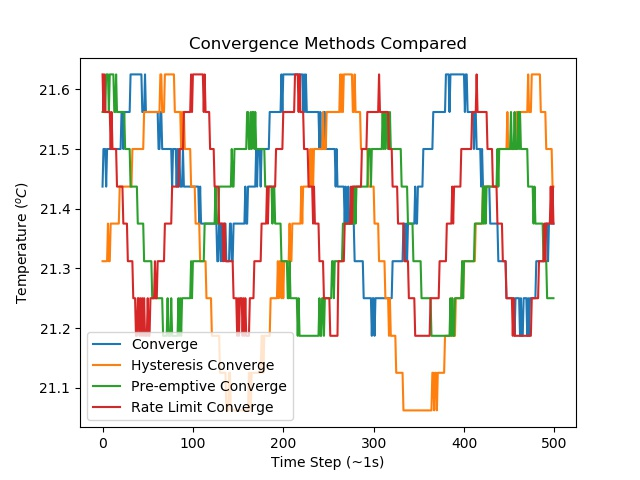
\includegraphics[scale=0.75]{comparison.jpg}
    \caption{\it{Here the convergence data for all of the convergence methods used can be seen together. This mainly shows the differences in the amplitudes of the different methods.}}
    \label{fig:comparison}
\end{figure}

\section{Python 3.6 Control Script}
All scripts for the running of the system used along with some scripts used for plotting and data analysis can be found at:

\centering https://github.com/Darthmazgar/Precision-Refrigerator-

% \newpage
% \section{Python Data Analysis Code}\label{ap:code}

% \lstdefinestyle{mystyle}{
    % backgroundcolor=\color{backcolour},   
    % commentstyle=\color{codegreen},
    % keywordstyle=\color{magenta},
    % numberstyle=\tiny\color{codegray},
    % stringstyle=\color{codepurple},
    % basicstyle=\footnotesize,
    % breakatwhitespace=false,         
    % breaklines=true,                 
    % captionpos=b,                    
    % keepspaces=true,                 
    % numbers=left,                    
    % numbersep=5pt,                  
    % showspaces=false,                
    % showstringspaces=false,
    % showtabs=false,                  
    % tabsize=2
% }
 
% \lstset{style=mystyle}
 
% \begin{document}
% \lstinputlisting[language=python]{}
% \end{document}

\end{document}